The exact `quasi-optimal' scheme for building a tensor train is TT-SVD~\cite{tensortrain}.

In~\cref{fig:ttsequence} we see the first step in the creation of a tensor train for a 4-way tensor. 

\begin{figure}
  \centering 
  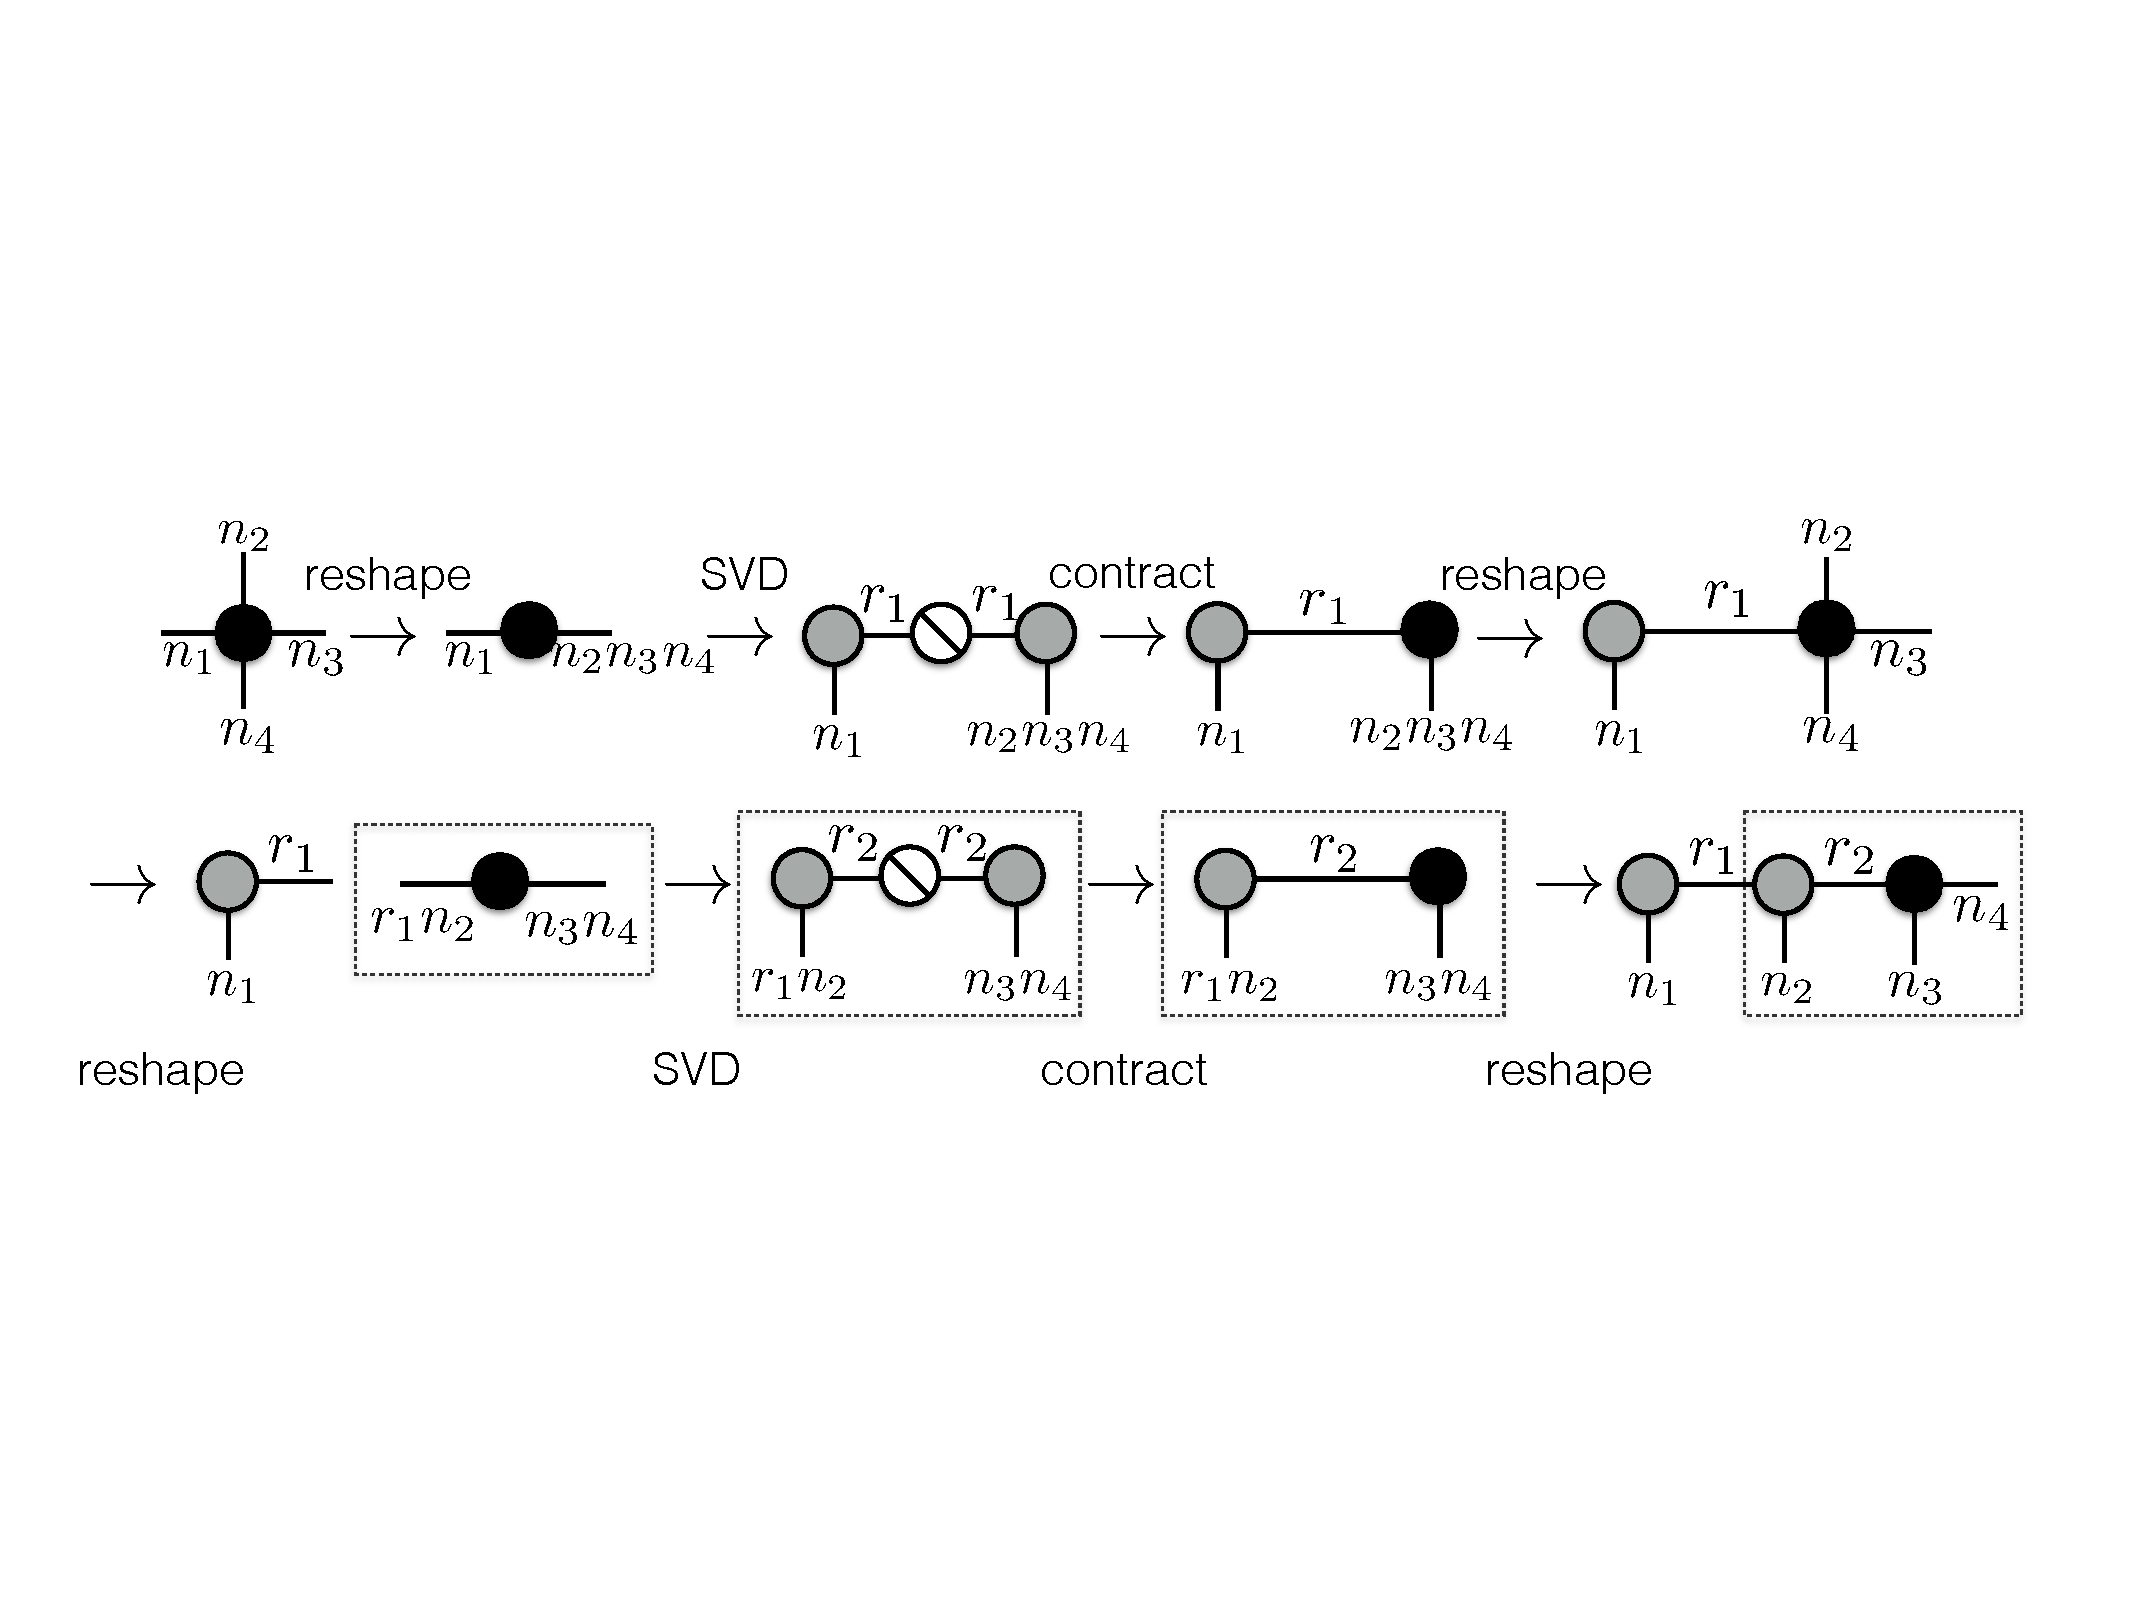
\includegraphics[width=\linewidth]{thpropfigs/ttsequence}
  \caption{The creation of the first two `carriages' of a tensor train decomposition for a 4-way tensor.}
  \label{fig:ttsequence}
\end{figure}

\paragraph{Proposal}
We summarize our proposed contributions as follows:
\begin{itemize}
  \item Implement the first distributed-memory implementation of the tensor train decomposition.
  \item Analyze the communication and computation behavior of the `reshape-SVD' method in distributed memory.
  \item Apply methods from our randomized Tucker decomposition to the tensor train in distributed memory.
  \item Benchmark both methods on a supercomputer and analyze/establish tradeoffs.
\end{itemize}